\documentclass[12pt]{article}
\usepackage[utf8]{inputenc}
\usepackage[T1]{fontenc}
\usepackage[norsk]{babel}
\usepackage{amsmath}
\usepackage{amsthm}
\usepackage{amsfonts}
\usepackage{amssymb}
\usepackage{enumerate}
\usepackage{physics}
\usepackage{graphicx}
\usepackage{wrapfig}
\usepackage{float}

\usepackage[top=0.2in, bottom=0.2in, left=0.2in, right=0.2in]{geometry} % Reduce margins
\newcommand{\mean}[1]{\langle #1 \rangle}


\begin{document}
\section{Energi i termofysikk}
\subsection{Ideell gass}
For lav-tetthets gasser gjelder
\begin{align*}
  PV = NkT = nRT
\end{align*}
\subsection{Ekvipartisjon av energi}
Gjelder for alle energiformer der formelen er en kvadratisk funksjon av koordinat-
eller hastighetskomponent. Dersom det i et system er $N$ molekyler med $f$
frihetsgrader hver, ingen ikke-kvadratiske temperaturavhengige former for energi
er den midlere (totale for store $N$) termiske energien gitt ved
\begin{align*}
  U_\text{termisk} = N f \frac{1}{2}kT
\end{align*}
Tar ikke hensyn til for eksempel hvileenergi, så tryggest å bruke for endringer
i energi med endringer i temperatur, og unngå tilfeller med faseoverganger
eller andre reaksjoner der kjemiske bindinger frigjør/krever energi.

\subsubsection{Telling av frihetsgrader}
Telling av frihetsgrader. Monoatomisk gass: Kun translasjonell bevegelse i tre
dimensjoner gir frihetsgrader, så $f = 3$. Diatomisk gass: Translasjonell
bevegelse i 3D + rotasjon om to akser (aksen gjennom lengden av molekylet
teller ikke pga. kvantemekanikk), så $f = 5$. Polyatomiske molekyler kan som
regel roteres om tre akser, som gir det siste rotasjonsbidraget. Vibrasjon
gir både kinetisk og potensiell energi bidrag, altså øker frihetsgraden med to.
Ved romtemperatur bidrar ikke vibrasjon til termisk energi, ved høyere temperaturer
kommer dette bidraget inn.

I et fast stoff kan atomer vibrere i tre ortogonale retninger, som gir 6 frihetsgrader.
Noen av disse kan "fryses ut" ved romtemperatur. Væsker er som regel mer kompliserte,
ekvipartisjonsteoremet gjelder for translasjonell bevegelse, men ikke for andre
bidrag siden de er ikke-kvadratiske.

\subsection{Varme og arbeid}
Overføringer av energi klassifiseres på to måter: \newline \noindent
\textbf{Varme}: overføring av energi fra et objekt til et annet på grunn av innbyrdes forskjell i temperatur. Ledning (molekylær
kontakt), konveksjon (bevegelse av områder av gass/væske) og elektromagnetisk stråling.\newline \noindent
\textbf{Arbeid} er enhver annen overføring av energi inn eller ut av et system.
\newline \noindent
Endringen i energi for et system er summen av varme og arbeid (termodynamikkens første lov)
\begin{align*}
  \Delta{U} = Q + W
\end{align*}
\subsection{Kompresjonsarbeid}
Arbeid som behøves for å redusere et volum av gass (trykk $P$) $\Delta V$ ved
\textbf{kvasistatisk} kompresjon (gassen rekker hele tiden å justere til likevekt).
\begin{align*}
  W = -P \Delta{V} \quad (\text{ved } P \neq P(V))\qquad W = - \int_{V_i}^{V_f} P(V) \dd V \quad (\text{ved } P = P(V))
\end{align*}
To idealiserte kompresjonstyper for ideell gass: \textbf{isotermal kompresjon}
(så sakte at temperatur i gassen er uendret) og \textbf{adiabatisk kompresjon}
(så kjapp at ingen varme slipper ut av systemet i prosessen). \newline \noindent
\textbf{Isotermal kompresjon}: Kvasistatisk, så
\begin{align*}
  W = -\int_{V_i}^{V_f} P \dd V = -NkT \int_{V_i}^{V_f} \frac{1}{V} \dd V = NkT \ln{\frac{V_i}{V_f}}
\end{align*}
Samme energi slipper ut ved varme (vises med første lov).\newline \noindent
\textbf{Adiabatisk kompresjon}: Ingen varme unnslipper, $\Delta U = Q + W = W$.
Bruk ekvipartisjon $\dd U = \frac{f}{2} N k \dd T$ og kvasistatisk kompresjon,
bruk ideell gass lov for trykket og løs separabel difflign. Får (med $\gamma = f(f+2)$)
\begin{align*}
  V T^{f/2} = \text{constant} \overset{\text{Ideell gass lov}}{\implies} V^\gamma P = \text{constant}
\end{align*}
\subsection{Varmekapasiteter}
Varmekapasitet defineres som $C = Q/\Delta{T}$ (varme per grad temperaturøkning). Tvetydig,
avhenger av omstendigheter (mengde stoff/gass, arbeid osv.). Derfor har man
varmekapasitet med $W = 0$ (som regel er $V$ da konstant, ingen kompressjon):
\begin{align*}
  C_V = \left( \frac{\Delta U}{\Delta T} \right)_V = \left( \pdv{U}{T}\right)_V
\end{align*}
Ofte ekspanderer gasser når de varmes opp, da tapes energi ved arbeid på omgivelsene.
Dersom det er konstant trykk i omgivelsene er
\begin{align*}
  C_P = \left( \frac{\Delta U - (-P\Delta V)}{\Delta T} \right)_P =  \left( \pdv{U}{T}\right)_P + P\left( \pdv{V}{T}\right)_P
\end{align*} \newline \noindent
\textbf{Latent varme:} Ved faseoverganger øker ikke temperaturen ved tilførsel av energi. Da
er varmekapasiteten per def uendelig: $C = Q/\Delta{T} = Q/0 = \infty$. Energien som kreves
for å fullføre faseoverangen kalles den latente varmen $L = Q/m$, og er varmen per
masse som kreves.\newline \noindent
\textbf{Entalpi:} Entalpi er energien til et system + ekspansjonsarbeidet som
krevdes for å putte det i det systemet det er i: $H = U + PV$. Observer at
$C_P = \left( \pdv{H}{T} \right)_P$.
\subsection{Prosesshastigheter (rates of processes)}
Vanligvis behøves ikke tiden det tar et system å nå likevekt å betraktes for å
finne likevektstiden. Dette nevnes allikevel kort her.
\subsubsection{Varmeledning}
Avhenger av en rekke faktorer, hvilke mekanismer er tilgjengelige. Hvis tomt
rom skiller objekter kan kun stråling lede varme. I et fluid er konveksjon
som regel dominant. Konveksjonstid funksjon av varmekapasitet og en rekke
faktorer som krefter, ganske komplisert. Den tredje måten er ved direkte
ledning, molekylær kontakt. Skjer i fast stoff og fluid former. I tilfellet
med to stoff med temperaturer $T_1$ og $T_2$ adskilt av f.eks glass med
tykkelse $\Delta x$, areal $A$ og som leder en varme $Q$ i løpet av en tid $\Delta t$.
\textbf{Fouriers varmeledningslov} sier at
\begin{align*}
  \frac{Q}{\Delta t} = - k_t A \frac{\dd T}{\dd x}
\end{align*}
der $k_t$ kalles \textbf{termisk konduktivitet} og er avhengig av materialet
varmen ledes gjennom, f.eks glass.
\subsubsection{Konduktiviteten til en ideell gass}
\subsubsection{Viskositet}
Momentum kan også spre seg gjennom et fluid. Situasjon med to parallele plater
med fluid imellom (dynamisk viskositet $\eta$ eller $\mu$). Platene beveger seg med ulike hastigheter.
Ved dimensjonsanalyse/logisk tenkning (evt. Navier-Stokes) er den viskøse motstandskraften
gitt ved
\begin{align*}
  \frac{|F_x|}{A} = \mu \frac{\dd u_x}{\dd z}
\end{align*}
\subsubsection{Diffusjon}

\section{Termodynamikkens andre lov}
\subsection{To tilstands systemer - paramagnetisme}
\textbf{Mikrotilstand} er alle partiklenes tilstander, \textbf{makrotilstand} sier
noe mer generelt om systemet. Multiplisiteten $\Omega(s)$ til en makrotilstand $s$ er antallet mikrotilstander
tilhørende makrotilstanden. Sannsynligheten for en makrotilstand er $\Omega(s)/\Omega(\text{alle})$. I en
to-tilstands paramagnet kan spinnene peke opp eller ned, $N = N_\uparrow + N_\downarrow$ er det totale antallet
spinn.
\begin{align*}
  \Omega(N_\uparrow) = \binom{N}{N_\uparrow} = \frac{N!}{N_\uparrow! (N - N_\uparrow)!} = \frac{N!}{N_\uparrow N_\downarrow}
\end{align*}
\subsection{Einsteinmodellen for faste stoffer}
System med et vilkårlig antall energi "enheter", alle med samme størrelse. Dette
er tilfellet for harmonisk oscillator, med steg $hf$ (Referansenivå settes til 0).
Disse oscillatorene gjelder for atomene i faste stoffer, 3 oscillatorer per atom
pga frihetsgrader. Multiplisiteten til Einstein solid med $N$ oscillatorer og
$q$ energi enheter er
\begin{align*}
  \Omega(N,q) = \binom{q + N - 1}{q} = \frac{(q + N - 1)!}{q!(N-1)!}
\end{align*}
\subsection{Interagerende systemer}
Har nå to Einstein solids, $A$ og $B$, som kan dele energi. Systemene uavhengige
av hverandre, så for en gitt energifordeling er multiplisiteten $\Omega_\text{tot} = \Omega_A \Omega_B$.\newline \noindent
\textbf{Fundamental antagelse i statistisk mekanikk:} I et isolert system i termisk
likevekt er enhver tilgjengelig mikrotilstand like sannsynlig. Merk at denne antagelsen
forutsetter at tidsskalaen er mye større enn tiden energiforskyvninger skjer. \newline \noindent
Observerer at multiplisiteten er langt høyere for de jevnere fordelingene av energi,
så med antagelsen over må en måling av jevn fordeling være overveldende sannsynlig.
\textbf{Termodynamikkens andre lov}(versjon 1): Multiplisiteten øker når et system
er for seg selv, fordi det er overveldende sannsynlig.
\subsection{Store systemer}
\subsubsection{Veldig store tall}
\textbf{Små tall:} 2,6,98. \textbf{Store tall:} Eksponentiering av små tall, f.eks
Avogadros tall $\sim 10^{23}$. Regneregel: $10^{23} + 23 = 10^{23}$.
\textbf{Veldig store tall:} Eksponentiering av store tall, f.eks $10^{10^{23}}$.
Regneregel: $10^{10^{23}} \times 10^{23} = 10^{(10^{23} + 23)} = 10^{10^{23}}$.
Logartime gjør et veldig stort tall til et stort tall osv, dette brukes mye.
\subsubsection{Stirlings Approksimasjon}
\begin{align*}
  N! \approx N^N e^{-N}\sqrt{2\pi N}
\end{align*}
Korrekt i grensen $N \gg 1$. God approksimasjon for logaritmen er gitt som $\ln{N!} \approx N \ln N - N$.
\subsubsection{Multiplisiteten til et stort Einstein solid}
Bruk Stirling på multiplisiteten til Einstein solid, med en rekkeutvikling av en
logaritme underveis. I grensen $q \gg N$ fåes
$\Omega(N,q) \approx \left(\frac{eq}{N}\right)^N$
\subsubsection{Skarpheten til multiplisitetsfunksjonen}
For to interagerende Einstein solids med $q \gg N$ er $\Omega = \left(\frac{e}{N}\right)^{2N} (q_A q_B)^{2N}.$
Har en skarp topp ved $\Omega = (e/N)^{2N} (q/2)^{2N}$, altså $q_A = q_B = q/2$,
en lik fordeling av energi. Fordelingen er Gaussisk og bredden er gitt ved $q/\sqrt{N}$.
For store $N$ vil fluktuasjoner være umulige å måle, denne grensen kalles den \textbf{termodynamiske grensen}.
\subsection{Ideell gass}
Utledning viser at $\Omega(U,V,N) \approx f(N) V^N U^{3N/2}$, der $f(N) = \frac{1}{N!} \frac{1}{h^{3N}} \frac{\pi^{3N/2}}{(3N/2)!} (2m)^{3N/2}$.
Kombineres to av disse (kun energiutveksling) fåes $\Omega_\text{total} = [f(N)]^2 (V_A V_B)^2 (U_A U_B)^{3N/2}$,
samme type uttrykk som for Einstein solid. Smal peak med høye multiplisiteter.
\subsection{Entropi}
Definerer entropi som (fordi multiplisitet er et veldig stort tall, og store tall er enklere å jobbe med)
\begin{align*}
  S = k \ln{\Omega}
\end{align*}
Dimensjon energi per temperatur, enhet $J/K$. En nyttig egenskap: $S_\text{tot} = k \ln{\Omega_\text{tot}} = k \ln{(\Omega_A \Omega_B)} = S_A + S_B$. \newline \noindent
\textbf{Termodynamikkens andre lov:} Ethvert stort system i likevekt vil være i
makrotilstanden med størst entropi (utenom fluktuasjoner som vanligvis er for små
til å måle). Altså: Entropi har en tensens til å øke.
\\ \\
Entropi kan ikke reduseres, enhver reduksjon i entropi i et system har skapt
mer entropi utenfor systemet.
\subsubsection{Entropi for en ideell gass}
\subsubsection{Blandingsentropi}
\section{Interaksjoner og implikasjoner}
\subsection{Temperature}
Se på system med to Einstein solids med noen hundre oscillatorer hver som deler
100 enheter energi. Plott entropi (individuelle og total) mot energi. Observer at
ved likevekt er $\pdv{S_A}{U_A} + \pdv{S_B}{U_A} = 0 \implies \pdv{S_A}{U_A} = \pdv{S_B}{U_B}$.
Dvs. det som er likt for begge systemer når de er i likevekt er stigningstallet til
entropi mot energigrafene, som da må ha noe med temperatur å gjøre (siden det er slik
temperatur er definert). Observer videre at det systemet med lav energi (da har det andre høy energi)
har en brattere $S$ mot $U$ graf, så en økning i energi skaper mer entropi enn det
høy energi systemet mister, så denne prosessen skjer av seg selv ifølge den andre loven.
Høyt stigningstall korresponderer med lav temperatur, og lavt med høy temperatur. Dette gir:
\begin{align*}
  \frac{1}{T} = \left(\pdv{S}{U} \right)_{N,V}
\end{align*}
\subsection{Entropi og varme}
\subsubsection{Finne termodynamiske størrelser for et system}
\begin{enumerate}
  \itemsep0em
  \item Bruk kvantemekanikk og/eller kombinatorikk til å finne et uttrykk for
  multiplisiteten som funksjon av $U,V,N$ og/eller andre variable. Må ofte bruke
  Stirlings approksimasjon og se på grenser.
  \item Ta logaritmen for å finne entropien.
  \item Deriver entropi mhp. energi for å finne temperatur som funksjon av $U$
  og evt. andre variable.
  \item Deriver $U(T)$ med hensyn på $T$ for å finne varmekapasiteten (med andre
  variable holdt konstant). Gjør andre operasjoner for å finne andre variable.
\end{enumerate}
\subsubsection{Måle entropier}
\subsubsection{Makroskopisk syn på entropi}
\subsection{Paramagnetisme}
$N$ spin 1/2 dipoler. $N_\uparrow: q = -\mu B$ og $N_\downarrow: q = \mu B$.
Total energi $U = N_\uparrow(-\mu B) + N_\downarrow \mu B = \mu B(N_\downarrow - N_\uparrow) = \mu B(N - 2N_\uparrow)$.
Magnetisering $M = \mu(N_\uparrow - N_\downarrow) = \frac{-U}{B}$. Brukes Stirling
på multiplisitetsfunksjonen og stegene over fåes $U = -N\mu B\tanh{\left(\frac{\mu B}{kT} \right)}$.
\subsection{Mekanisk likevekt og trykk}
Hva med når systemer $A$ og $B$ kan utveksle både energi og volum? Utveksling av
energi skjer på grunn av temperaturer, utveksling av volum styres av trykk.
Ved likevekt er $\pdv{S}{V_A} = 0$ (også ingen endring med hensyn på energi). Trykket
må være likt i begge sider ved likevekt, og ved stor endring i entropi per endring i
volum vil trykket være stort, gassen ønsker å ekspandere. Relasjonen blir
\begin{align*}
  P = T \left( \pdv{S}{V} \right)_{U,N}
\end{align*}
\subsubsection{Den termodynamiske identiteten}
Anta det skjer en prosess på et system der energien og volumet endres med $\Delta U$
og $\Delta V$ (volum konstant under energiendring, energi konstant under volumendring).
Prosessen kan deles opp i to steg, og endringen i entropi er gitt ved summen av
endringene fra de to prosessene. Så ved identitetene over er
\begin{align*}
  \dd S = \left( \pdv{S}{U} \right)_{V} \dd U + \left( \pdv{S}{V} \right)_{U}\dd V
\end{align*}
Dette kalles \textbf{den termodynamiske identiteten}, og skrives ofte om til (merk
at disse ligningene forutsetter at andre variable, som $N$, holdes konstant)
\begin{align*}
  \dd U = T \dd S - P \dd V
\end{align*}
\subsubsection{Entropi og varme igjen}
Uttrykket over ligner veldig på $\dd U = Q + W$ (termodynamikkens første lov).
Sammenligningen gjelder så lenge volumendringer skjer kvasistatisk og andre
størrelser er konstante (f.eks $N$). Da er $W = -P \dd V$, så $Q = T \dd S$,
selv om det gjøres arbeid på systemet. I tilfellet der endringen er adiabatisk $Q = 0$
og kvasistatisk er entropien uendret. Dette kalles en \textbf{isentropisk} prosess.
\subsection{Diffusiv likevekt og kjemisk potensial}
To systemer i termisk likevekt har like temperaturer. Mekanisk likevekt tilsvarer
like trykk. Hva med diffusiv likevekt? Betrakt to systemer som kan utveksle
partikler og energi, men er under konstant volum. Antar samme "art", f.eks $\text{H}_2\text{O}$,
men tilstandsformer er vilkålig. Antar total energi og antall partikler er konstant,
så ved likevekt er $\left( \pdv{S}{U_A} \right)_{N_A, V_A} = 0$ og $\left( \pdv{S}{N_A} \right)_{U_A, V_A} = 0$.
Ved likevekt er $\pdv{S}{N_A} = \pdv{S}{N_B}$ ved konstant energi og volum. Ganger opp
med temperatur og definerer det kjemiske potensialet
\begin{align*}
  \mu \equiv - T \left(\pdv{S}{N} \right)_{U,V}
\end{align*}
Systemer overlatt til seg selv vil dermed gå mot lavere kjemiske potensial, siden
dette gir høyere entropi. Altså strømmer partikler fra systemer med høyere $\mu$
til lavere.

Vi kan nå utvide den termodynamiske identiteten ytterligere. Total endring i entropi
ved å endre $U$ med $\dd U$, $P$ med $\dd P$ og $N$ med $\dd N$ er
\begin{align*}
  \dd S &= \left( \pdv{S}{U} \right)_{N, V} \dd U + \left( \pdv{S}{V} \right)_{N, U} \dd V + \left( \pdv{S}{N} \right)_{U, V} \dd N\\
        &= \frac{1}{T} \dd U + \frac{P}{T} \dd V + \mu \dd N
\end{align*}
Eller, løst for $\dd U$ fåes
\begin{align*}
  \dd U = T \dd S - P \dd V + \mu \dd N
\end{align*}
De to siste leddene kalles vanligvis henholdsvis mekanisk og kjemisk arbeid, det
første leddet er som tidligere varme. Dersom det er flere typer partikler/atomer
har de hvert sitt kjemiske potensial, da erstattes det siste leddet av en sum
av $\mu_i \dd N_i$ ledd.
\section{Motorer og kjølemaskiner}
\subsection{Varmekraftmaskiner}
\begin{wrapfigure}{R}{0.3\textwidth}
  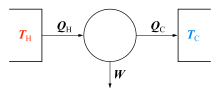
\includegraphics[width=0.3\textwidth]{figures/carnot.png}
\end{wrapfigure}
En \textbf{varmekraftmaskin} er et apparat som absorberer varme og omdanner
deler av energien til arbeid. Et eksempel er dampturbinen. Grunnen til at kun
deler av energien kan omdannes er at når varme strømmer inn kommer det også
entropi, og denne må en kvitte seg med før prosessen kan starte om.
Varme kommer fra det \textbf{varme reservoiret} $T_H$ og varmen som dumpes dumpes til
det \textbf{kalde reservoiret} $T_C$. Arbeidet motoren gjør er $W$. Alle størrelsene er positive.
Effektivitet defineres som arbeid ut per varme inn
\begin{align*}
  e \equiv \frac{W}{Q_h}
\end{align*}
Hvordan maksimere effektiviteten? Energibevaring gir $Q_h = Q_c + W$, som gir
effektiviteten $e = \frac{Q_h - Q_c}{Q_h} = 1 - Q_c/Q_h$.
Videre, entropien i systemet kan ikke bli mindre, så $Q_c / T_c \geq Q_h / T_h$.
Settes dette inn i effektivitetsuttrykket over får man $e \leq 1 - T_c / T_h$.
Velg $T_c$ og $T_h$ slik at forholdet blir så lite som mulig. Den første loven
sier 'du kan ikke vinne', og den andre loven sier at 'du går uansett i underskudd'.
\begin{wrapfigure}{R}{0.5\textwidth}
  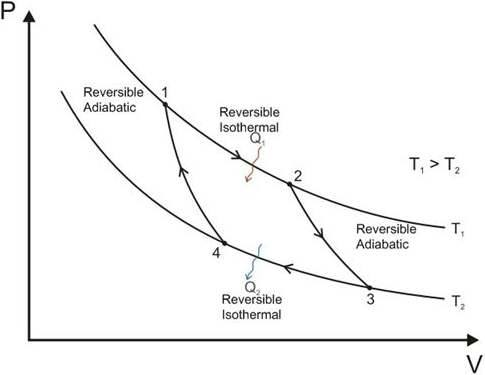
\includegraphics[width=0.5\textwidth]{figures/carnotPV.jpg}
\end{wrapfigure}
\subsubsection{Carnotsyklusen}
Hvordan lage en motor som oppnår maksimal effektivitet for gitt $T_h$ og $T_c$?
Enhver motor har væske/gass som transporterer energien. Først ønsker vi at
gassen tar imot varme $Q_h$ fra det varme reservoiret, da synker entropien i
reservoiret med $Q_h/T_h$, og entropien øker i gassen med $Q_h / T_\text{gass}$.
For å unngå å lage mer entropi må $T_h = T_g$, men det går ikke, da transporteres
ingen energi ved varme. Så sett $T_g$ litt lavere enn $T_h$, og hold den ved
denne temperaturen når den varmes ved å la den ekspandere. Dette steget krever
isoterm ekspansjon av gassen.

Når gassen dumper varme til det kalde reservoiret vil vi temperaturen kun skal
være infinitesimalt større enn $T_c$ for å lage minst mulig entropi. Og når varmen
forlater la gassen komprimere isotermalt for å holde den ved denne temperaturen.
Vi har altså isotermal ekspansjon ved temperatur litt mindre enn $T_h$ og isotermal
kompressjon rett over $T_c$. Hvordan få gassen fra en temperatur til den andre og
så tilbake? Vi ønsker ingen utveksling av varme i disse stegene, så de må være
adiabatiske. Stegene er altså: 1: Isotermal ekspansjon ved $T_h$. 2: Adiabatisk ekspansjon
fra $T_h$ til $T_c$. 3: Isotermal kompressjon ved $T_c$. 4: Til slutt adiabatisk kompressjon tilbake til $T_h$.

\subsection{Kjølemaskiner}
Kjølemaskiner er varmekraftmaskiner kjørt baklengs. Varme går fra det kalde
reservoiret til det varme ved tilførsel av arbeid som elektrisk energi. Kjøleskapet
er det kalde reservoiret og systemet utenfor det varme. 'Søppelvarme' dumpes ut
i kjøkkenet. COP (coefficient of performance) defineres som
\begin{align*}
  \text{COP} = \frac{\text{benefit}}{\text{cost}} = \frac{Q_c}{W}
\end{align*}
Kan som over bruke første og andre lov til å vise begrensninger for COP.
\section{Fri energi og kjemisk termodynamikk}
\subsection{Fri energi som tilgjengelig arbeid}
\textbf{Entalpi} er energien til et system pluss arbeided som behøves for å lage plass ved å dytte
atomosfære/annet med trykk $P$ vekk. Altså energi som trengs hvis systemet
skal dannes ut av intet og plasseres i et annet system:
\begin{align*}
  H \equiv U + PV
\end{align*}
\textbf{Helmholtz fri energi} er energien som trengs for å lage et system, minus
varmen man får 'gratis' fra omliggende atmosfære med temperatur $T$. Ekvivalent er
dette energien som kan hentes ut dersom systemet annihileres, entropi kan ikke minke
så entropi må dumpes ut som varme. $F$ er da energien man får ut som arbeid:
\begin{align*}
  F \equiv U - TS
\end{align*}
\textbf{Gibbs fri energi} er en kobinasjon av de over.
\begin{align*}
  G \equiv U - TS + PV
\end{align*}
Som regel betraktes ikke situasjoner der hele systemet annihileres, så det er
bedre å se på endringer i størrelsene over. Da er $\Delta F = \Delta U - T \Delta S = Q + W - T \Delta S$.
Dersom ingen entropi dannes er $Q = T\Delta S$, og $\Delta F = W$. Dersom entropi
dannes er $T\Delta S > Q$, og $\Delta F < W$, så ved konstant temperatur er
\begin{align*}
  \Delta F \leq W
\end{align*}
Samme argumentasjon for konstant trykk og temperatur og at $W = -P\Delta V + W_\text{annet}$
gir
\begin{align*}
  \Delta G \leq W_\text{annet}
\end{align*}
\subsubsection{Elektrolyse, brenselceller og batterier}
Et eksempel på bruk av $\Delta G$, betrakt reaksjonen $\text{H}_2 \text{O} \rightarrow \text{H}_2 + \frac{1}{2}\text{O}_2$,
elektrolyse av vann til hydrogen og oksygengass. Fra tabell er $\Delta H = 286$ kJ (energien man ville fått dersom man brant et mol hydrogen).
I denne reaksjonen må denne energien altså tilføres, $P\Delta V = 4$ kJ av energien går til å dytte atmosfære vekk, resten blir værende i systemet.
Hvor mye må tilføres ved arbeid og hvor mye ved varme? Fra tabeller er $S_{\text{H}_2 \text{O}} = 70 \text{ J/K}$, $S_{\text{H}_2} = 131 \text{ J/K}$
og $S_{\text{O}_2} = 205 \text{ J/K}$. Endring i entropi er $\Delta S = S_1 - S_0 = (131 + 0.5 \cdot 205) - 70 = 163$ J/K, entropien øker. Maksimal
energiendring ved varme er da $T\Delta S = 49$ kJ. Energien som behøves via elektrisk arbeid
er forskjellen $286 - 49 = 237$ kJ. Dette er endringen i Gibbs fri energi, det minste arbeidet som behøves for
å få reaksjonen til å gå: $\Delta G = 237 \text{ kJ} = \Delta H - T \Delta S = 286 \text{ kJ} - (298 \text{ K})(163 \text{ J/K})$.
\subsubsection{Termodynamiske identiteter}
Kan lage identiteter for de overnevnte energiene, betrakt små endringer i $H, U, P$ og $V$
og bruk den termodynamiske identiteten til å eliminere $\dd U$. Gir
\begin{align*}
  \dd H &= T \dd S + V \dd P + \mu \dd N \\
  \dd F &= -S \dd T - P \dd V + \mu \dd N \\
  \dd G &= -S \dd T + V \dd P + \mu \dd N
\end{align*}
Fra disse kan en rekke partiellderiverte relasjoner finnes. For eksempel
\begin{align*}
  S = -\left( \pdv{G}{T} \right)_{P,N}
\end{align*}
kan lages ved å bruke den siste og holde $P$ og $N$ konstant, dvs $\dd P = \dd N = 0$.
\subsection{Fri energi som kraft mot likevekt}
\textbf{Reservoir} av energi: System stort nok til at det kan utveksle uendelig
energi uten å endre sin temperatur. \newline \noindent
Betrakt et system i kontakt med et reservoir $R$ av uendelig størrelse, slik at
det kan slippe uendelige mengder energi uten å endre sin temperatur. Total entropi
for universet blir $S + S_R$. Husk at entropi har en tendens til å øke, betrakt
liten endring i entropi $\dd S_\text{tot} = \dd S + \dd S_R$. Bruker termodynamisk identitet $\dd S = \dd U /T + \dd V P/T - \dd N \mu /T$
for reservoiret og antar konstant volum og antall partikler, så endringen i entropi kan skrives $\dd S_\text{tot} = \dd S + \dd U_R / T_R$.
Men temperaturene i systemet og reservoiret er like, så energiutvekslingene må være like. Så
\begin{align*}
  \dd S_\text{tot} = \dd S - \frac{1}{T} \dd U = - \frac{1}{T}(\dd U - T\dd S) = - \frac{1}{T} \dd F
\end{align*}
Konklusjon: Med konstant $T, V, N$ tilsvarer økning i $S$ for universet en minking
av $F$ (Helmholz fri energi) for systemet! Tilsvarende, ved å la trykket være lik reservoiret og
lar volumet variere finner man at $\dd S_\text{tot} = -\frac{1}{T}\dd G$, så Gibbs fri
energi har en tendens til å minke for systemet. Oppsummering:
\begin{itemize}
  \item Ved konstant energi og volum tendenserer entropien $S$ til å øke.
  \item Ved konstant temperatur og volum tendenserer $F$ til å minke.
  \item Ved konstant temperatur og trykk tendenserer $G$ til å minke.
\end{itemize}
Litt intuisjon om dette, $F \equiv U - TS$, så under konstant temperatur er minking av
$F$ tilsvarende økning av $S$ (som gir mening jf. andre lov i termo) og minking i $U$. Dette
gir intuitivt mening, men hvorfor? Når systemet gir opp energi går denne energien til
omgivelsene, som fører til en økning i entropi (dette er viktigst for små $T$, mens systementropi viktigst for større $T$).
Tilsvarende betraktninger gjelder for Gibbs fri energi.
\subsubsection{Extensive and intensive quantities}
Dersom man kopierer et system og setter det sammen med det originale systemet til
et nytt system, vil noen variable dobles og noen forbli uendret. Variablene som dobles
kalles \textbf{ekstensive} egenskaper, mens variablene som ikke endrer seg er \textbf{intensive}.
Ekstensive egenskaper er $V, N, S, U, H, F, G, \text{masse}$, mens intensive egenskaper er eksempelvis
$T, P, \mu, \text{tetthet}$.
\subsubsection{Gibbs fri energi og kjemisk potensial}
Husker at $\mu = \left(\pdv{G}{N}\right)_{T,P}$. $T$ og $P$ (intensive størrelser) holdes
konstant, så dersom vi legger til en partikkel øker $G$ med $\mu$. Dette er fordi $G$ må
vokse i proporsjon med $N$ når de intensive egenskapene holdes konstant. Derfor er
\begin{align*}
  G = N \mu \text{ som sier at det kjemiske potensialet er Gibbs fri energi per partikkel}
\end{align*}
Det samme argumentet gjelder ikke for $\mu = \left(\pdv{F}{N}\right)_{T,V}$, siden
tettheten endrer seg og da vil $\mu$ endre seg. Dette kommer av at $V$ er en ekstensiv størrelse.
Generalisering av uttrykket over blir $G = \sum_i N_i \mu_i$ når det er flere typer partikler.
\subsection{Faseoverganger}
En \textbf{faseovergang} er en diskontinuerlig endring i egenskapene til et stoff
når noe rundt bare endres infinitesimalt. Et \textbf{fasediagram} viser likevektsfaser
kom funksjon av trykk og temperatur. Trykket der en gass kan sameksistere med flytende
fase kalles \textbf{damptrykket}. Punktet (kombinasjonen av $P$ og $T$) der
alle tre faser sameksisterer kalles \textbf{trippelpunktet}. Ved lavere temperaturer
kan ikke væskeformen eksistere, fast stoff sublimerer til gass.

Ta med eksempler på fasediagrammer. Skriv kort om Heliumene og magnetisk system.
\subsubsection{Diamanter og grafitt}

\subsubsection{Clausius-Clapeyron relasjonen}
Gir stigningstallet til faseovergangsgrensegrafen i et PT-diagram. Ved faseovergangen
er materialet like stabilt som væske som gass, så Gibbs fri energi må være lik uansett
fase: $G_l = G_g$. (Tilsvarende: Væske og gass i diffusiv likevekt - kjemisk potensial per partikkel
(Gibbs fri energi) må være like).
Øk så temperaturen og trykket med $\dd T$ og $\dd P$ slik at de to fasene er like
stabile, da må Gibbs fri energi endre seg like mye for begge: $\dd G_l = \dd G_g$.
Utvider dette med termodynamisk identitet: $-S_l \dd T + V_l \dd P = -S_g \dd T + V_g \dd P$
($\mu \dd N$ leddet ikke med siden $N$ konstant). Dette gir ($\Delta S = S_g - S_l = L/T$ der $L$ er latent varme)
\begin{align*}
  \dv{P}{T} = \frac{S_g - S_l}{V_g - V_l} = \frac{L}{T \Delta V} \quad \text{Clausius-Clapeyron. Gjelder for alle fasegrenser.}
\end{align*}
\subsubsection{Van der Waals modellen}
\section{Boltzmann statistikk}
\subsection{Boltzmann faktoren}
\textbf{Degenerert:} Flere uavhengige tilstander som tilsvarer samme energinivå.
Betrakt atom med energinivåer og i kontakt med reservoir. Hva er sannsynligheten
for at atomet er i tilstanden $s_1$ eller $s_2$? Tilstandene har energier $E(s_1)$
og $E(s_2)$ og sannsynligheter $P(s_1)$ og $P(s_2)$. Atomet og reservoiret er
et lukket system, så alle tilgjengelige mikrotilstander like sannsynlige. Har tilsvarende
multiplisiteten til reservoiret ved disse tilstandene: $\Omega_R(s_1)$ og $\Omega_R(s_2)$.
Logikk tilsier at
\begin{align*}
  \frac{P(s_2)}{P(s_1)} = \frac{\Omega_R(s_2)}{\Omega_R(s_1)} = \frac{e^{S_R(s_2)/k}}{e^{S_R(s_1)/k}} = e^{[S_R(s_2) - S_R(s_1)]/k} = \frac{e^{-E(s_2)/kT}}{e^{-E(s_1)/kT}}
\end{align*}
Eksponenten  nest siste likhet er endring i entropi. Bruker termodynamisk identitet $\dd S_R = 1/T (\dd U_R + P \dd V_R - \mu \dd N_R)$,
kaster bort de siste to leddene (entropiendring som følge av volumendring neglisjerbar i forhold til energitilstandsendring, og
antallet partikler er konstant). Kan skrive om entropiendringene til energiendringer, får siste likhet over. Faktorene i siste
uttrykk kalles Boltzmann faktorer, disse er sannsynligheter så lenge de normaliseres med en partisjonsfunksjon $Z$.
\begin{align*}
  P(s) = \frac{1}{Z} e^{-E(s)/kT}
\end{align*}
Observasjoner: Sannsynligheten går ned for høyere energis tilstander.
\subsubsection{Partisjonsfunksjonen}
Har ved loven om total sannsylighet (setter ofte $\beta = 1 / kT$)
\begin{align*}
  Z = \sum_s e^{-\beta E(s)}
\end{align*}
\subsection{Forventningsverdier (gjennomsnittsverdier)}
\begin{align*}
  \mean{X} = \sum_s X(s) P(s) = \sum_s X(s) e^{-\beta E(s)}
\end{align*}
Husk at forventningsverdier er additive, trenger bare å regne ut gjennomsnittlig
energi til en partikkel og gange med antallet partikler for å finne total energi.
\subsection{Ekvipartisjonsteoremet - Bevis}
Anta kvadratiske frihetsgrader, dvs $E(q) = c q^2$ der $c$ er en konstant og $q$
er en romlig eller momentum koordinat ($x$, $p_x$ og $L_x$ er eksempler). Anta
tilstandene er $\approx$infinitesimalt diskretisert i deler $\Delta q$. Har
$Z = \sum_q e^{-\beta E(q)} = \sum_q e^{-\beta c q^2} = \frac{1}{\Delta q}\sum_q e^{-\beta c q^2}\Delta q$.
Approksimerer summen som et integral, bytte variabel til $x = \sqrt{\beta c q}$ med $\dd q = \dd x / \sqrt{\beta c}$.
Får $Z = \frac{1}{\Delta q} \frac{1}{\sqrt{\beta c}} \int_{-\infty}^{\infty} e^{-x^2} \dd x = C \beta^{-1/2}$ der $C = \sqrt{\pi/c}/\Delta q$.
Forventningsverdien til energi er da gitt som (dette blir ekvipartisjonsteoremet)
\begin{align*}
  \mean{E} = -\frac{1}{Z} \pdv{Z}{\beta} = \hdots = \frac{1}{2}kT
\end{align*}
Gjelder ikke for kvantemekaniske systemer siden antallet distinkte tilstander
som har signifikante sannsynligheter blir for liten, og integralapproksimasjonen
blir dårlig. Gjelder ikke for lave temperaturer, siden for få tilstander har
store nok bidrag.
\subsection{Maxwells hastighetsfordeling - utledning}
Ønsker å finne sannsynlighetstetthet for molekylhastigheter i en ideell gass. Forventer at
tettheten $D$ oppfyller følgende proporsjonalitet
\begin{align*}
  D(v) \propto (\text{Sannsynlighet for å ha hastighet } \vb v) \times (\text{Antall vektorer $\vb v$ som finnes for en hastighet $v$}) = 4\pi v^2 e^{-mv^2 / 2kT}
\end{align*}
Den første faktoren finnes enkelt ved at energien er $mv^2 / 2$, så proporsjonaliteten
til sannsynligheten er gitt ved Boltzmannfaktoren $e^{-mv^2 / 2kT}$. Den andre
finnes ved å betrakte arealet til sfæren av mulige momentum vektorer, som har areal
$4\pi v^2$. Proporsjonalitetskonstanten er effektivt en normaliseringskonstant. Denne kan regnes ut til resultatfordelingen
\begin{align*}
  D(v) = \left( \frac{m}{2\pi k T} \right)^{3/2} 4\pi v^2 e^{-mv^2 /2kT}
\end{align*}
\subsection{Partisjonsfunksjoner og fri energi}
\begin{align*}
  F = -kT \ln{Z} \qquad Z = e^{-F/kT}
\end{align*}
Fra denne kan entropi, trykk og kjemisk potensial regnes ut:
\begin{align*}
  S = -\left( \pdv{F}{T} \right)_{V,N} \qquad P = -\left( \pdv{F}{V} \right)_{T,N} \qquad \mu = \left( \pdv{F}{N} \right)_{T,V}
\end{align*}
\subsection{Partisjonsfunksjoner for sammensatte? (composite) systems}
Hvordan relateres $Z$ for et system til $Z$ for hver partikkel? Betrakter først system med
to partikler. Hvis disse ikke interagerer med hverandre er den totale energien $E_1 + E_2$, og
\begin{align*}
  Z_\text{tot} = \sum_s e^{-\beta[E_1(s) + E_2(s)]} = \sum_s e^{-\beta E_1(s)} e^{-\beta E_2(s)}
\end{align*}
der summen er over alle tilstandene til det sammensatte systemet. Hvis, i tillegg,
partiklene er adskillbare er tilstandene for det sammensatte systemet ekvivalent med
settet med alle mulige par av tilstander
\begin{align*}
  Z_\text{total} = \sum_{s_1}\sum_{s_2} e^{-\beta E_1(s_1)} e^{-\beta E_2(s_2)} = \sum_{s_1} e^{-\beta E_1(s_1)} \sum_{s_2} e^{-\beta E_2(s_2)} = Z_1 Z_2 \\
  \text{(Distinguishable, noninteracting particles)}
\end{align*}
Hvis partiklene er ikke-adskillbare er
\begin{align*}
  Z_\text{total} = \frac{1}{2}Z_1 Z_2\qquad \text{(Noninteracting, undistinguishable particles)}
\end{align*}
Denne er ikke helt korrekt ettersom det er noen ledd i dobbeltsummen over der begge
partiklene er i samme tilstand, disse ble ikke telt dobbelt og burde ikke kuttes bort. I ideell
gass og lignende systemer er sjansene for at to partikler er i samme tilstand neglisjerbare.
Generelt, for $N$ partikler er
\begin{align*}
  Z_\text{total} = Z_1 Z_2 \hdots Z_N \qquad \text{($N$ noninteracting, distinguishable particles)} \\
  Z_\text{total} = \frac{1}{N!} Z_1^N \qquad \text{($N$ noninteracting, indistinguishable particles)}
\end{align*}
\subsection{Ideell gass med partisjonsfunksjonbetraktning}
Hvert molekyl kan ta opp en masse forskjellige tilstander, partisjonsfunksjonen for
hver partikkel er $Z_1$, og systemets partisjonsfunksjon er $Z = Z_1^N / N!$, siden
partiklene er ikke skillbare. Boltzmannfaktorene er på formen $e^{-E(s)/kT} = e^{-E_\text{tr}(s)/kT} e^{-E_\text{int}(s)/kT}$,
der energien er delt i translasjonell og indre (rotasjon, vibrasjon eller whatever) energi.
Summen av tilstander kan skrives som en dobbeltsum over translasjonell og indre bidrag, så $Z_1 = Z_\text{tr} Z_\text{int}$.

\textbf{Translasjonell del:} Hver partikkel i boks (infinite square well). Løsninger
sinusoidale med $\lambda_n = 2L / n$ for heltallige $n$ som gir $p_n = h / \lambda = hn/2L$.
Energiene blir $E_n = \frac{p_n^2}{2m} = \frac{h^2 n^2}{8mL^2}$. Putt disse energiene
inn i Boltzmannfaktorer og regn ut translasjonell partisjonsfunksjon. $Z_\text{1d} = \sum_n e^{-E_n / kT} = \sum_n e^{-h^2 n^2 / 8mL^2 kT}$.
Så lenge $L$ og/eller $T$ ikke er kjempesmå er energinivåene veldig tett på hverandre,
approksimerer summen som et integral. $\ell_Q$ kalles kvantelengden, utenom $\pi$-faktoren
er den De Broglie bølgelengden til en partikkel med masse $m$ og energi $kT$.
\begin{align*}
  Z_\text{1d} = \int_0^\infty e^{-h^2 n^2 / 8mL^2 kT} \dd n = \sqrt{\frac{2\pi m k T}{h^2}}L \equiv \frac{L}{\ell_Q}
\end{align*}
For en realistisk boks er dette er veldig stort tall, ergo er det mange tilstander tilgjengelig.
I tre dimensjoner er summen en sum over $n_x$, $n_y$ og $n_z$ av produktet av boltzmannfaktorer med $n_x$ osv.
Dette blir et tredimensjonalt integral som kan skrives som produktr av integralet over, resultatet er
$\frac{L_x}{\ell_Q}\frac{L_y}{\ell_Q}\frac{L_z}{\ell_Q} = \frac{V}{v_Q}$. Her er $v_Q = \ell^3$ kvantevolumet.

Med disse resultatene har vi for en partikkel $Z_1 = \frac{V}{v_Q} Z_\text{int}$,
hvor den indre partisjonsfunksjonen er en sum over indre tilstander. For hele gassen med $N$ molekyler
er $Z = \frac{1}{N!} \left( \frac{V Z_\text{int}}{v_Q} \right)^N$. Logaritmen er $\ln Z = N[\ln V + \ln Z_\text{int} - \ln N - \ln v_Q + 1]$.
\subsubsection{Utregning av andre størrelser}
\begin{align*}
  U   &= - \frac{1}{Z}\pdv{Z}{\beta} = -\pdv{\beta} \ln{Z} = -N \pdv{\beta} Z_\text{int} + \frac{N}{v_Q} \pdv{v_Q}{\beta} = N \mean{E_\text{int}} + N \frac{3}{2}\frac{1}{\beta} = U_\text{int} + \frac{3}{2}NkT \\
  C_V &= \pdv{U}{T} = \pdv{U_\text{int}}{T} + \frac{3}{2}Nk
\end{align*}
For en diatomisk gass er det indre bidraget til varmekapasiteten fra rotasjon og vibrasjon, som begge legger til om lag $Nk$ til
varmekapasiteten ved høye nok temperaturer, og går til $0$ ved lave temperaturer. I teorien
forsvinner det translatoriske bidraget ved lave temperaturer, men bare hvis $\ell_Q \sim L$, så
å bytte om til et integral fra summen over blir feil. Andre størrelser:
\begin{align*}
  F   &= -kT\ln{Z} = -NkT[\ln V + \ln Z_\text{int} - \ln{N} - \ln{v_Q} + 1] = -NkT [\ln V + \ln Z_\text{int} - \ln{N} - \ln{v_Q} + 1] + F_\text{int} \\
  P   &= \left( \pdv{F}{V} \right)_{T,N} = \frac{NkT}{V} \qquad
  S   = \left( \pdv{F}{T} \right)_{V,N} = Nk \left[ \ln{\left( \frac{V}{v_Q N} \right)} + \frac{5}{2} \right] - \pdv{F_\text{int}}{T} \qquad
  \mu = \left( \pdv{F}{N} \right)_{T,V} = -kT \ln{\left( \frac{V Z_\text{int}}{N v_Q} \right)}
\end{align*}
\section{Kvantestatistikk}
\subsection{Gibbsfaktoren}
Samme utledning som for Boltzmannfaktoren, men denne gangen kan systemet utveksle
partikler med reservoiret, det er i diffusiv likevekt. Tar med $\mu \dd N$ leddet
fra termodynamisk identitet, endring for reservoiret er lik endring for systemet, får
faktorer på formen
\begin{align*}
  P(s) = \frac{1}{\mathcal{Z}} e^{-[E(s) - \mu N(s)]/kT} \qquad \text{der } \mathcal{Z} = \sum_s e^{-[E(s) - \mu N(s)]/kT}
\end{align*}
kalles \textbf{Gibbs summen} og summen går over alle mulige tilstander (inkludert alle mulige verdier for $N$).
Dersom det er flere typer partikler blir $\mu \dd N$ leddet en sum over $\mu_i \dd N_i$, og Gibbs faktoren blir
$e^{-[E(s) - \mu_A N_A(s) - \mu_B N_B(s)]/kT}$ for et tilfelle med to typer partikler.
\subsubsection{Eksempel: Karbonmonoksidforgiftning}

\subsection{Bosoner og Fermioner}
Gibbsfaktorer sin viktigste anvendelse er i \textbf{kvantestatistikk}. Da er det ofte
så få mulige tilstander eller så høy tetthet at det er en betydelig sannsynlighet
for at identiske partikler ønsker å ta opp samme en-partikkels tilstand. Partisjonsfunksjonen
for system med $N$ ikke-skillbare, ikke-interagerende partikler $Z = Z_1^N / N!$ i forrige
kapittel gjelder kun når ingen partikler er i samme tilstand.

Noen partikler kan oppta samme tilstand. Patikler som kan dele samme tilstand
med hverandre kalles \textbf{bosoner} (for eksempel fotoner, pioner, helium-4 atomer).
Mange partikler kan ikke dele samme tilstand, disse kalles \textbf{fermioner}, og
eksempler er elektroner, protoner, osv. Regelen som sier dette kalles \textbf{Paulis eksklusjonsprinsipp}.
Partikler med heltalls spinn er bosoner, halvtallige spinn er fermioner.

I mange tilfeller er det irrelevant om partiklene er bosoner eller fermioner. Dette gjelder
når antallet tilgjengelige tilstander er langt større enn antallet partikler $Z_1 \gg N$.
Med uttrykket for enpartikkels partisjonsfunksjon for ideell gass blir kravet $V/N \gg v_Q$
der $V$ er volumet til gassen, $N$ er antallet partikler og $v_Q$ er kvantevolumet (omtrent
den gjennomsnittlige de Broglie bølgelengden i tredje potens). Altså må gjennomsnittlig
avstand mellom partiklene være mye større enn den gjennomsnittlige de Broglie bølgelengden.
Når avstandene blir for små og kravet ikke holder vil bølgefunksjonene begynne å overlappe,
og oppførselen blir helt annerledes enn for en ideell gass. Veldig høy tetthet eller
lave temperaturer gjør at dette skjer.
\subsubsection{Distribusjonsfunksjoner}
Betrakter en-partikkel tilstanden til et system som har energi $\epsilon$ når
en partikkel tar den opp og energi $0$ når den ikke er tatt opp. Sannsynligheten
for at den er tatt opp av $n$ partikler er
\begin{align*}
  P(n) = \frac{1}{\mathcal{Z}} e^{-(n\epsilon - \mu n)/kT} = \frac{1}{\mathcal{Z}} e^{-n(\epsilon - \mu)/kT}
\end{align*}
Gibbs summen er enkel dersom partiklene er fermioner, $\mathcal{Z} = 1 + e^{-(\epsilon - \mu)/kT}$.
Forventningsverdien til antallet tilstander tatt opp (kalles \textbf{okkupans}) er
\begin{align*}
  \mean{n} = \sum_n n P(n) = \frac{e^{-n(\epsilon - \mu)/kT}}{1 + e^{-(\epsilon - \mu)/kT}} = \frac{1}{e^{(\epsilon - \mu)/kT} + 1}
\end{align*}
Dette kalles \textbf{Fermi-Dirac fordelingen}.

Dersom partiklene er bosoner kan $n$ være ethvert ikke-negaivt heltall, så Gibbs summen er
\begin{align*}
  \mathcal{Z} = 1 + e^{-(\epsilon - \mu)/kT} + e^{-2(\epsilon - \mu)/kT} + \hdots = 1 + e^{-(\epsilon - \mu)/kT} + (e^{-(\epsilon - \mu)/kT})^2 + \hdots = \frac{1}{1-e^{-(\epsilon - \mu)/kT}}
\end{align*}
Gjennomsnittlig antall partikler i tilstanden er (sett $x = (\epsilon - \mu)/kT$)
\begin{align*}
  \mean{n} = \sum_n n P(n) = \sum_n n \frac{e^{-nx}}{\mathcal{Z}} = - \frac{1}{\mathcal{Z}} \sum_n \pdv{x} e^{-nx} = \frac{1}{\mathcal{Z}} \pdv{\mathcal{Z}}{x} = \frac{1}{e^{(\epsilon - \mu)/kT} - 1}
\end{align*}
Dette kalles \textbf{Bose-Einstein fordelingen}. Begge disse fordelingene reduserer til Boltzmannfordelingen
i grensen der $\epsilon \gg \mu$.
\subsection{Degenererte Fermi gasser}
Betrakter elektroner, men det under gjelder for alle fermioner. Temperatur så lav
at kravet $V/N \gg v_Q$ er langt unna å være oppfylt. For et elektron ved
romtemperatur er $v_Q = (h / \sqrt{2\pi m k T})^3 = (4.3 \text{ mm})^3$. I et metall
er volumet per ledningselektron $(0.2\text{nm})^3$, så temperaturen er for lav til
at Boltzmannstatistikk kan anvendes. Vi betrakter derfor det motsatte tilfellet,
og setter i første omgang $T = 0$.
\subsubsection{Temperatur lik null}
Fermi-Dirac fordelingen blir en step-function. Alle enpartikkel tilstander med
energi mindre enn $\mu$ er tatt opp, alle tilstander med større energi er ikke
tatt opp. Her kalles $\mu$ for \textbf{Fermi energien}, skrevet $\epsilon_F \equiv \mu(T = 0)$.
Når en elektrongass er så kalt at nesten alle tilstandene under $\epsilon_F$ er tatt opp, mens alle
over ikke er det, kalles \textbf{degenerert} (ikke relatert til vanlig bruk av ordet i QM).

Verdien til $\epsilon_F$ bestemmes av antallet elektroner tilstede. Tom boks,
legg til et elektron av gangen, hvert nye elektron går da til den laveste
tilgjengelige tilstanden, til det siste elektronet går i en tilstand rett under
$\epsilon_F$. Å legge til et elektron må få en energi $\epsilon_F$, siden $\mu = \left( \pdv{U}{N} \right)_{S,V}$
og $\dd U = \mu$ når $\dd N = 1$.

Approksimasjon: Ingen andre krefter i det hele tatt utenom at de er fanget i en boks med $V = L^3$,
for ledningselektroner i et metall er dette ikke en god approksimasjon på grunn av
tiltrekkende krefter fra ioner i krystallen. For elektron i en boks er bølgefunksjonene
sinusoidale med $\lambda_n = 2L/n$ og $p_n = h/\lambda_n = hn/2L$. I tre dimensjoner
er det en slik for hver dimensjon, tillatte energier er derfor $\epsilon = \vb p^2 / 2m = \frac{h^2}{8mL^2} (n_x^2 + n_y^2 + n_z^2)$.

\subsubsection{Små temperaturer større enn null}
\begin{align*}
  U = \frac{3}{5} N \epsilon_F + \frac{\pi^2}{4} N \frac{(kT)^2}{\epsilon_F} \implies C_V = \left( \pdv{U}{T} \right) = \frac{\pi^2 N k^2 T}{2\epsilon_F}
\end{align*}
\subsubsection{Tetthet av tilstander}

\subsection{Sort legeme stråling}
\section{Viktigste formler + annet nyttig}
\subsection{Summer/integraler}
\begin{align*}
  \sum_{k = 0}^{n} r^k &= \frac{1 - r^{n+1}}{1 - r} \quad \text{Sum av endelig geometrisk rekke}\\
  \sum_{k = 0}^{\infty} r^k &= \frac{1}{1-r} \qquad \text{Sum av uendelig geometrisk rekke (mye brukt for partisjonsfunksjoner/Gibbssummer)} \\
  \int_{-\infty}^\infty e^{-x^2} \dd x &= \sqrt{\pi}
\end{align*}
\subsection{Kombinatorikk}
1. To operasjoner som kan gjøres på $n$ og $m$ måter kan kombineres på $m \cdot n$ måter.
2. Antall ordnede utvalg med tilbakelegging av $r$ elementer fra en mengde med $n$ elementer er $n^r$.
3. Antall ordnede utvalg uten tilbakelegging av $r$ elementer fra en mengde med $n$ elementer er $n(n-1)\hdots (n-r+1) = n!/(n-r)!$.
4. Antall måter $n$ elementer kan ordnes i rekkefølge på (permuteres) er $n! = (1)(2)\hdots(n-1)(n)$.
\begin{align*}
  \binom{n}{r} = \frac{n!}{r!(n-r)!} \quad \text{Antall ikke-ordnede utvalg av $r$ elementer fra en mengde med $n$ elementer} \\
  \binom{n}{n_1 n_2 \hdots n_r} = \frac{n!}{n_1! n_2! \hdots n_r!} \quad \text{Antall måter $n$ elementer kan deles inn i $r$ delmengder med $n_i$ elementer}
\end{align*}
\subsection{Viktigste formler}
Termodynamikkens tre lover (energibevaring, entropi øker og $S \rightarrow 0$ når $T \rightarrow 0$):
\begin{align*}
  \Delta E = Q + W \qquad \Delta{Q} = T \delta{S} \qquad S = k \ln{\Omega}, T = 0 \rightarrow \Omega = 1 \rightarrow S = 0
\end{align*}
Termodynamiske identiteter
\begin{align*}
  \dd U &= T \dd S - P \dd V + \mu \dd N \\
  \dd H &= T \dd S + V \dd P + \mu \dd N \\
  \dd F &= -S \dd T - P \dd V + \mu \dd N \\
  \dd G &= -S \dd T + V \dd P + \mu \dd N
\end{align*}
Fri energi og partisjonsfunksjon relasjon
\begin{align*}
  F = -kT \ln{Z} \qquad Z = e^{-F/kT}
\end{align*}
\begin{align*}
  \mean{U} = - \frac{1}{Z} \pdv{Z}{\beta}
\end{align*}
\section{Kort om forsøkene vi hadde! }
\end{document}
